\documentclass[__main__.tex]{subfiles}

\begin{document}

\qtitle{Э}{12}
Сила Ампера. Момент сил, действующих на виток с током в однородном магнитном поле. Магнитный момент тока. Гипотеза молекулярных токов Ампера. Намагниченность.\\ 

\textbf{Сила ампера}\\

\begin{wrapfigure}{L}{.3\linewidth}
	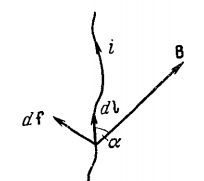
\includegraphics{e-03-amper}
	\caption{Сила Ампера}
	\label{e-12-force}
\end{wrapfigure}
Согласно закону Ампера на элемент тока $d\vec{I}$ действует в магнитном поле сила
\begin{gather}
d\vec{f} = kid\vec{I} \times \vec{B},
\label{e-12-amper}
\end{gather}
где $k$ - коэффициент пропорциональности,\\
$i$ - сила тока,\\
$\vec{B}$ - магнитная индукция в том месте, где помещается элемент $dI$.\\
Величина силы \ref{e-12-amper} вычисляется по формуле 
\begin{gather}
df = kiBdl\sin{\alpha},
\end{gather}
где $\alpha$ - угол между векторами $d\vec{I}$ и $\vec{B}$. Сила направлена перпендикулярно к плоскости, в которой лежат $d\vec{I}$ и $\vec{B}$(рис.\ref{e-12-force}).\\

\textbf{Момент сил, действующих на виток с током в однородном магнитном поле}\\

\begin{wrapfigure}[16]{l!}{.4\linewidth}
	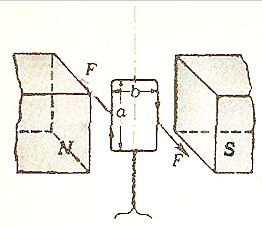
\includegraphics{e-12-frame}
	\caption{Прямоугольная рамка с током}
		\label{e-12-frame}
\end{wrapfigure}
Рамка помещена в однородное магнитное поле с индукцией $\vec{B}$ так, что в начальный момент вектор $\vec{B}$ лежит в плоскости рамки и параллелен двум ее сторонам. На боковые стороны(длиной $a$) действуют противонаправленные силы, равные по модулю $F = BIa$(закон Ампера). На остальные две стороны силы не действуют($\sin{\alpha} = 0$). Каждая из сил $\vec{F}$ относительно оси(рис.\ref{e-12-frame}), проходящей через середины верхней и нижней сторон рамки, создает момент силы (вращающий момент), равный  $\frac{BIab}{2}$ ($\frac{b}{2}$ — плечо силы). Знаки моментов одинаковы, так что общий вращающий момент $M$ равен $BIab$.
\begin{gather*}
	M = BIab = BIS (ab = S).
\end{gather*}
Под действием этого момента рамка начнёт поворачиваться(по часовой
стрелке, если смотреть сверху(рис.\ref{e-12-frame1})) и продолжит, пока её плоскость не будет перпендикулярна вектору индукции $\vec{B}$. В этом положении сумма сил и сумма моментов сил равны нулю, и рамка находится в состоянии устойчивого равновесия. В любом промежуточном положении, когда нормаль к плоскости контура составляет произвольный угол $\beta$ с индукцией магнитного поля, вращающий момент равен
\begin{gather}
	M = BIS\sin{\beta}
	\label{e-12-momentum}
\end{gather}
Из \ref{e-12-momentum} видно, что при данном значении $B$ и при определенном положении контура с током $M$ зависит только от $IS$. Величина $IS$ есть модуль вектора магнитного момента.\\
Векторно магнитный момент:
\begin{gather*}
\vec{p}_m = IS\vec{n},
\end{gather*}

\begin{wrapfigure}[14]{l!}{0.3\linewidth}
	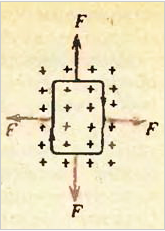
\includegraphics{e-12-frame1}
	\caption{Прямоугольная рамка с током. Вид сверху}
	\label{e-12-frame1}
\end{wrapfigure}
где $\vec{n}$ - нормаль к контуру. Работает правило буравчика(крутишь по направлению тока, двигаешься по направлению магнитного момента).\\
\textbf{Магнитный момент тока}
\begin{definition}[По википедии]
Магни́тный моме́нт, магни́тный дипо́льный моме́нт — основная величина, характеризующая магнитные свойства вещества.\\
\textit{Формулы}
\begin{gather*}
	\vec{p}_m = IS\vec{n}; \hspace{0.5cm}
	\vec{p}_m = \frac{I}{2}\oint{[\vec{r}, d\vec{l}]}; \hspace{0.5cm} \vec{p}_m = \frac{1}{2}\int_{V}{[\vec{r}, \vec{j}]dV}.
\end{gather*}
$\vec{n}$ - нормаль к плоскости контура,\; $S$ - площадь контура.\\
$\vec{r}$ - радиус-вектор от начала координат до элемента длины контура $d\vec{l}$, \; $\vec{j}$ - плотность тока в элементе объёма $dV$.	
\end{definition}
\textbf{Гипотеза Ампера}\\
Для объяснения намагничения тел Ампер предположил, что в молекулах вещества циркулируют круговые токи. Каждый такой ток обладает магнитным моментом и создаёт в окружающем пространстве магнитное поле. В отсутствие внешнего поля молекулярные токи ориентированы беспорядочным образом, вследствие чего обусловленное ими результирующее поле равно нулю. В силу хаотической ориентации магнитных моментов отдельных молекул суммарный магнитный момент тела также равен нулю. Под действием поля магнитные моменты молекул приобретают преимущественную ориентацию в одном направлении, вследствие чего магнетик намагничивается - его суммарный магнитный момент становится отличным от нуля. Магнитные поля отдельных молекулярных токов в этом случае уже не компенсируют друг друга и возникает поле $\vec{B'}$.\\
\textbf{Намагниченность}
\begin{definition}[википедия]
	Намагниченность — векторная физическая величина, характеризующая магнитное состояние макроскопического физического тела. Определяется как магнитный момент единицы объёма вещества:
	\begin{gather*}
		\vec{M} = \frac{\vec{p}_m}{V}
	\end{gather*}
\end{definition}
\begin{definition}[Савельев]
	Намагничение магнетика естественно характеризовать магнитным моментом единицы объёма. Эту величину называют \textit{вектором намагничивания}. Если магнетик намагничен неоднородно, вектор намагничения в данной точке:
	\begin{gather*}
		\vec{J} = \frac{\underset{\Delta V}{\sum}{\vec{p}_m}}{\Delta V},
	\end{gather*}
	где $\Delta V$ - физически бесконечно малый объём, взятый в окрестности рассматриваемой точки,\\
	$\vec{p}_m$ - магнитный момент отдельной молекулы.
\end{definition}
\textit{Связи с другими величинами}\\
$\vec{M} = \chi_m\vec{H}$ ($\chi_m$ - магнитная восприимчивость) -  формула не работает с ферромагнитами.\\\\
$\vec{B} = \mu_0(\vec{H} + \vec{M})$ (СИ) \hspace{0.5cm} $\vec{B} = (\vec{H} + 4\pi\vec{M})$ (СГС) -  связь с магнитной индукцией.
\end{document}